\documentclass{article}
\usepackage{graphicx}
\usepackage{amsmath}
\usepackage{amssymb}
\usepackage[margin=1in]{geometry}
\usepackage{float}
\usepackage{booktabs}

\title{Mass versus Velocity at the Characteristic Time: $N=4$, $8$, $16$}
\author{Kevin Bedoya}
\date{August 2026}

\begin{document}
\maketitle

\begin{figure}[H]
  \centering
  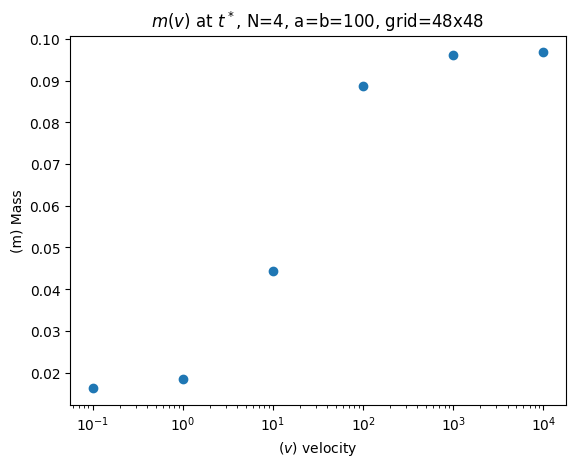
\includegraphics[width=0.75\textwidth]{figures/char_time/char_t_N4.png}
  \caption{Total mass as a function of filament velocity, $m(v)$, for $N=4$.
  Each point is captured at the characteristic time $t^{*}$ of its own run,
  not at a common time.}
\end{figure}

\begin{table}[H]
  \centering
  \begin{tabular}{ccc}
    \toprule
    $v$ & $t^{*}$ & $m^{*}$ \\
    \midrule
    $10^{-1}$ & $0.0853$ & $0.0162$ \\
    $10^{0}$ & $0.0845$ & $0.0186$ \\
    $10^{1}$ & $0.0775$ & $0.0443$ \\
    $10^{2}$ & $0.0709$ & $0.0888$ \\
    $10^{3}$ & $0.0702$ & $0.0961$ \\
    $10^{4}$ & $0.0701$ & $0.0968$ \\
    \bottomrule
  \end{tabular}
  \caption{Characteristic time $t^{*}$ and the mass $m^{*}$ captured at that
  respective $t^{*}$, per velocity $v$, for $N=4$ (3 significant figures).}
\end{table}

\clearpage

\begin{figure}[H]
  \centering
  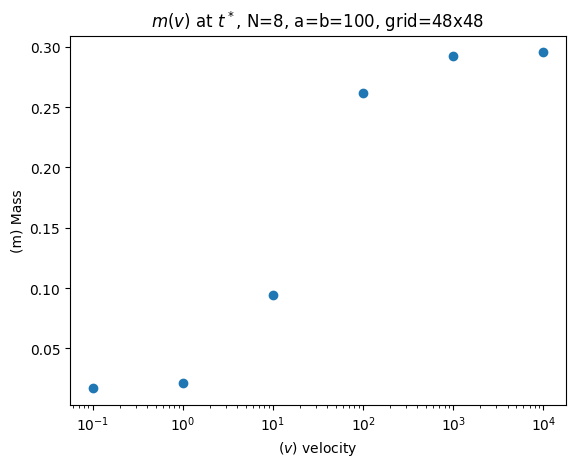
\includegraphics[width=0.75\textwidth]{figures/char_time/char_t_N8.png}
  \caption{Total mass as a function of filament velocity, $m(v)$, for $N=8$.
  Each point is captured at the characteristic time $t^{*}$ of its own run,
  not at a common time.}
\end{figure}

\begin{table}[H]
  \centering
  \begin{tabular}{ccc}
    \toprule
    $v$ & $t^{*}$ & $m^{*}$ \\
    \midrule
    $10^{-1}$ & $0.0914$ & $0.0169$ \\
    $10^{0}$ & $0.0901$ & $0.0216$ \\
    $10^{1}$ & $0.0771$ & $0.0941$ \\
    $10^{2}$ & $0.0636$ & $0.262$ \\
    $10^{3}$ & $0.0620$ & $0.292$ \\
    $10^{4}$ & $0.0618$ & $0.295$ \\
    \bottomrule
  \end{tabular}
  \caption{Characteristic time $t^{*}$ and the mass $m^{*}$ captured at that
  respective $t^{*}$, per velocity $v$, for $N=8$ (3 significant figures).}
\end{table}

\clearpage

\begin{figure}[H]
  \centering
  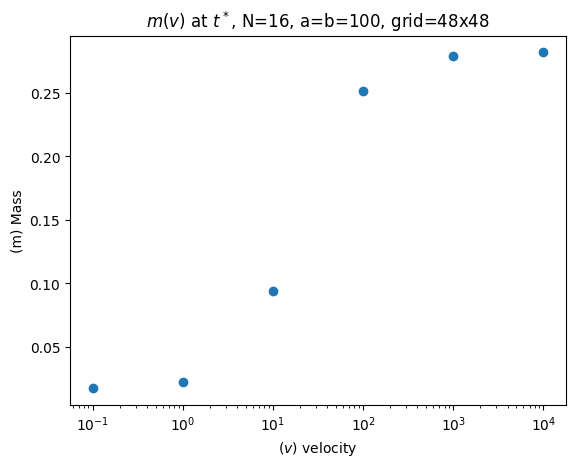
\includegraphics[width=0.75\textwidth]{figures/char_time/char_t_N16.png}
  \caption{Total mass as a function of filament velocity, $m(v)$, for $N=16$.
  Each point is captured at the characteristic time $t^{*}$ of its own run,
  not at a common time.}
\end{figure}

\begin{table}[H]
  \centering
  \begin{tabular}{ccc}
    \toprule
    $v$ & $t^{*}$ & $m^{*}$ \\
    \midrule
    $10^{-1}$ & $0.0913$ & $0.0170$ \\
    $10^{0}$ & $0.0900$ & $0.0218$ \\
    $10^{1}$ & $0.0770$ & $0.0937$ \\
    $10^{2}$ & $0.0642$ & $0.251$ \\
    $10^{3}$ & $0.0627$ & $0.279$ \\
    $10^{4}$ & $0.0625$ & $0.282$ \\
    \bottomrule
  \end{tabular}
  \caption{Characteristic time $t^{*}$ and the mass $m^{*}$ captured at that
  respective $t^{*}$, per velocity $v$, for $N=16$ (3 significant figures).}
\end{table}

\clearpage

\section*{A scaling factor in $m^{*}$ relating $N=4$ to $N=8$ and $N=16$}

All three sweeps were run at the same coupling ($a=b=100$), the same grid
($48\times48$), and over the same six velocities, so the three $m^{*}(v)$
trajectories can be placed on a common plot by a single constant per $N$.

Take the mass at the largest velocity of the sweep, $m^{*}_{N}(10^{4})$, as the
reference level. The scaling factor is its ratio to the $N=4$ value,
%
\begin{equation}
  \boxed{\;
  c_{N} \;=\; \frac{m^{*}_{N}(10^{4})}{m^{*}_{4}(10^{4})}\;}
  \label{eq:c}
\end{equation}
%
and each trajectory is brought onto the common curve by dividing through by it,
%
\begin{equation}
  \hat{m}^{*}_{N}(v) \;=\; \frac{m^{*}_{N}(v)}{c_{N}}.
  \label{eq:scaled}
\end{equation}

\begin{table}[H]
  \centering
  \begin{tabular}{ccc}
    \toprule
    $N$ & $m^{*}_{N}(10^{4})$ & $c_{N}$ \\
    \midrule
    $4$  & $0.09679$ & $1$ (reference) \\
    $8$  & $0.29547$ & $3.053$ \\
    $16$ & $0.28216$ & $2.915$ \\
    \bottomrule
  \end{tabular}
  \caption{Mass at $v=10^{4}$ and the resulting scaling factor of
  Eq.~\eqref{eq:c}.}
  \label{tab:c}
\end{table}

\begin{figure}[H]
  \centering
  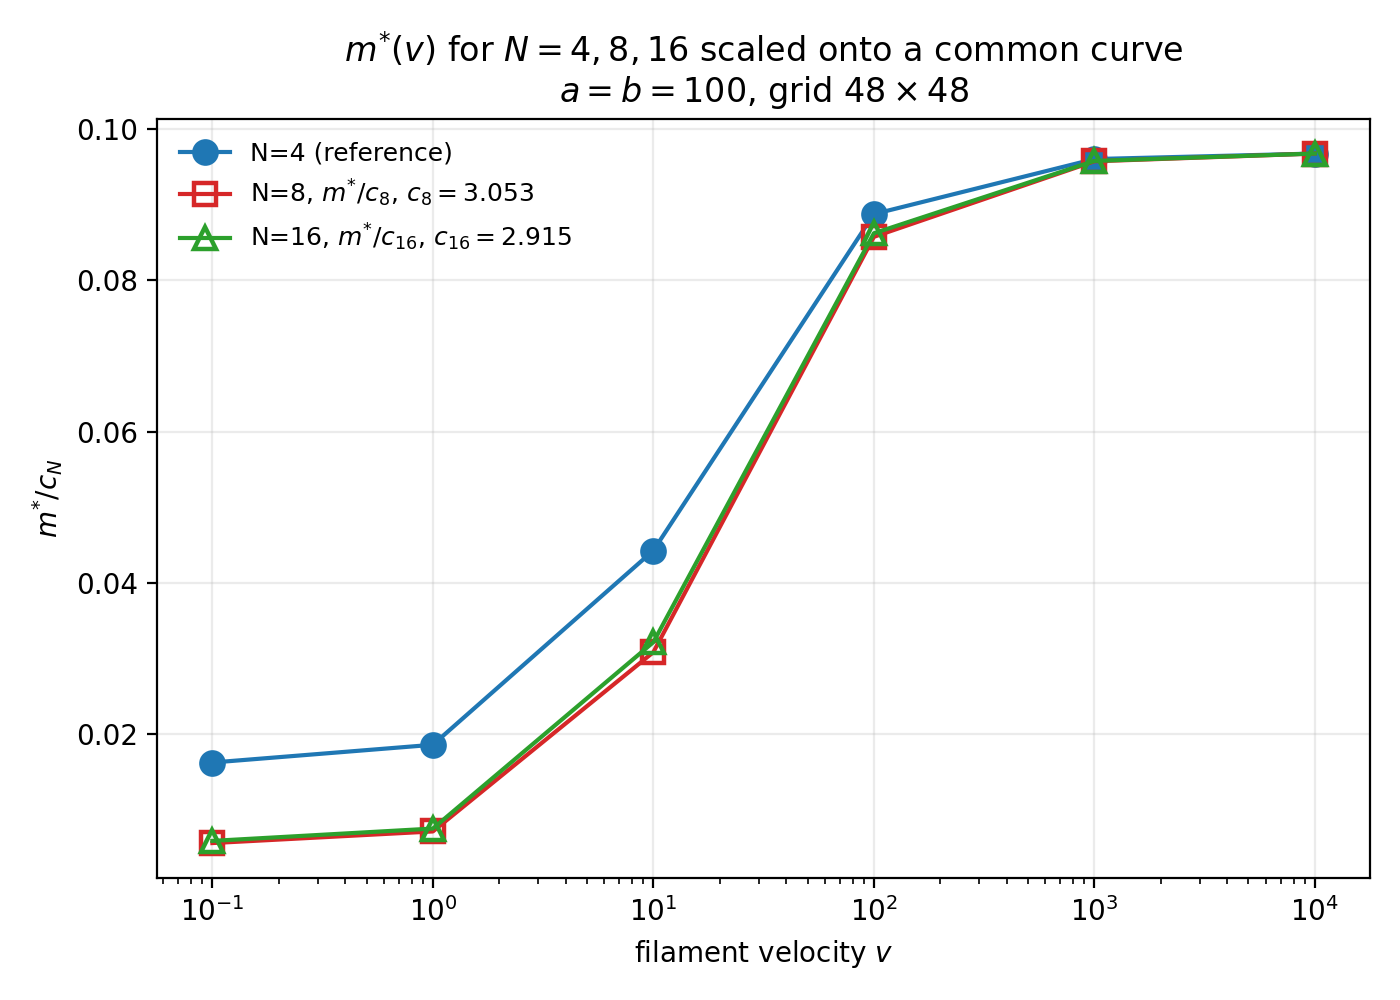
\includegraphics[width=0.85\textwidth]{figures/char_time/char_t_collapse_N4_N8_N16.png}
  \caption{The three trajectories after applying Eq.~\eqref{eq:scaled}, with
  the constants $c_{N}$ of Table~\ref{tab:c}. The curves lie together over the
  upper three decades of $v$; $N=8$ and $N=16$ coincide throughout. The
  separation at $v\lesssim 10^{0}$ is expected, since a single multiplicative
  constant fixed on the plateau cannot also match the low-velocity end.}
  \label{fig:collapse}
\end{figure}

\clearpage

\end{document}
